\documentclass[14pt]{extreport}
\usepackage[utf8]{inputenc}
\usepackage[english, russian]{babel}
\usepackage{listings}
\usepackage{graphicx}
\usepackage{float}
\graphicspath{{imgs/}}
\usepackage{amsmath,amsfonts,amssymb,amsthm,mathtools} 
\usepackage{pgfplots}
\usepackage{filecontents}
\usepackage{indentfirst}
\usepackage{eucal}
\usepackage{enumitem}
\frenchspacing

\usepackage{indentfirst} % Красная строка

\usetikzlibrary{datavisualization}
\usetikzlibrary{datavisualization.formats.functions}

\usepackage{amsmath}
\usepackage{fixltx2e}
\usepackage{caption}


\definecolor{bluekeywords}{rgb}{0,0,1}
\definecolor{greencomments}{rgb}{0,0.5,0}
\definecolor{redstrings}{rgb}{0.64,0.08,0.08}
\definecolor{xmlcomments}{rgb}{0.5,0.5,0.5}
\definecolor{types}{rgb}{0.17,0.57,0.68}

\usepackage{listings}
\lstset{language=[Sharp]C,
	captionpos=t,
	numbers=left, %Nummerierung
	numberstyle=\small, % kleine Zeilennummern
	frame=single, % Oberhalb und unterhalb des Listings ist eine Linie
	stepnumber=1,                   
	numbersep=5pt,                
	showspaces=false,
	tabsize=2,
	showtabs=false,
	breaklines=true,
	showstringspaces=false,
	breakatwhitespace=true,
	escapeinside={(*@}{@*)},
	commentstyle=\color{greencomments},
	morekeywords={partial, var, value, get, set},
	keywordstyle=\color{bluekeywords},
	stringstyle=\color{redstrings},
	basicstyle=\ttfamily\small,
}

\usepackage[left=1cm,right=1cm, top=1cm,bottom=2cm,bindingoffset=0cm]{geometry}
% Для измененных титулов глав:
\usepackage{titlesec, blindtext, color} % подключаем нужные пакеты
\definecolor{gray75}{gray}{0.75} % определяем цвет
\newcommand{\hsp}{\hspace{20pt}} % длина линии в 20pt
% titleformat определяет стиль
\titleformat{\chapter}[hang]{\Huge\bfseries}{\thechapter\hsp\textcolor{gray75}{|}\hsp}{0pt}{\Huge\bfseries}

\usepackage{array}
\newcommand{\head}[2]{\multicolumn{1}{>{\centering\arraybackslash}p{#1}}{#2}}

% plot
\usepackage{pgfplots}
\usepackage{filecontents}
\usetikzlibrary{datavisualization}
\usetikzlibrary{datavisualization.formats.functions}

\begin{document}
	%\def\chaptername{} % убирает "Глава"
	\thispagestyle{empty}
	\begin{titlepage}
		\noindent \begin{minipage}{0.15\textwidth}
			
\includegraphics[width=\linewidth]{b_logo}
		\end{minipage}
		\noindent\begin{minipage}{0.9\textwidth}\centering
			\textbf{Министерство науки и высшего образования Российской Федерации}\\
			\textbf{Федеральное государственное бюджетное образовательное учреждение высшего образования}\\
			\textbf{~~~«Московский государственный технический университет имени Н.Э.~Баумана}\\
			\textbf{(национальный исследовательский университет)»}\\
			\textbf{(МГТУ им. Н.Э.~Баумана)}
		\end{minipage}
		
		\noindent\rule{18cm}{3pt}
		\newline\newline
		\noindent ФАКУЛЬТЕТ $\underline{~~~~~~~~~~~~~~~~~~~~~~~~~~~~~~~\text{«Информатика и системы управления»}~~~~~~~~~~~~~~~~~~~~~~~~~~~~~~~~~~~~~}$ \newline\newline
		\noindent КАФЕДРА $\underline{~~~~~~~~~~~~~\text{«Программное обеспечение ЭВМ и информационные технологии»}~~~~~~~~~~~~~~~~~~~~~~~}$\newline\newline\newline\newline\newline\newline
		
		
		\begin{center}
			\noindent\begin{minipage}{1.3\textwidth}\centering
				\Large\textbf{  Отчет по лабораторной работе №6}\newline
				\textbf{по дисциплине \newline "Моделирование"}\newline\newline
			\end{minipage}
		\end{center}
		
		\noindent\textbf{Тема} $\underline{\text{Моделирование работы супермаркета}}$\newline\newline
		\noindent\textbf{Студент} $\underline{\text{Малышев И. А.}}$\newline\newline
		\noindent\textbf{Группа} $\underline{\text{ИУ7-71Б}}$\newline\newline
		\noindent\textbf{Оценка (баллы)} $\underline{\text{~~~~~~~~~~~~~~~~~~~~~~~~~~~}}$\newline\newline
		\noindent\textbf{Преподаватель: } $\underline{\text{Рудаков И. В.}}$\newline\newline\newline
		
		\begin{center}
			\vfill
			Москва~---~\the\year
			~г.
		\end{center}
	\end{titlepage}
	
	
	\setcounter{page}{2}

\chapter{Задание}

Реализовать программу для моделирования следующей системы: в супермаркете покупатели приходят к кассам с заданным интервалом времени. У каждой кассы формируется своя очередь. Клиент выбирает очередь с минимальной длинной. Кассиры обслуживают клиентов за заданный интервал времени. После того, как все товары отсканированы, клиенту необходимо оплатить товар. У каждого терминала оплаты формируется своя очередь. Клиент выбирает терминал с очередью наименьшей длины. Терминалы обслуживают клиентов за фиксированный интервал времени. Количество клиентов задается. 

\chapter{Решение}
\section{Теоретическая часть}

\subsection{Структурная схема системы в терминах СМО}

Структурная схема в терминах СМО представлена на рисунке \ref{img:model}.

\begin{figure}[H]
	\begin{center}
		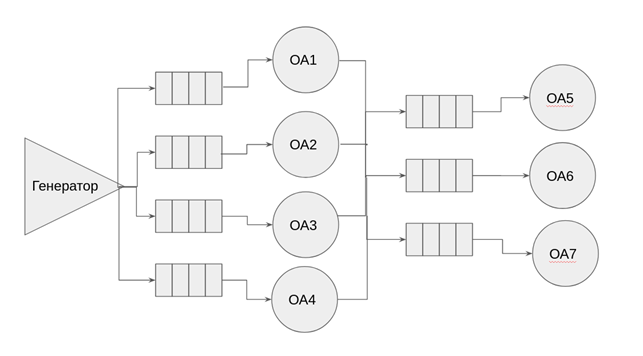
\includegraphics[scale=0.9]{imgs/model.png}
	\end{center}
	\caption{Структурная схема системы в терминах СМО.}
	\label{img:model}
\end{figure}

\section{Листинг}

Далее представлен фрагмент программы, выполняющий поставленное задание.

\begin{lstlisting}
from numpy import random as nr
	
class Generator:
	def __init__(self, generator, count):
		self._generator = generator
		self.receivers = []
		self.num_requests = count
		self.next = 0 
	
	def next_time(self):
		return self._generator.generate()
	
	def generate_request(self):
		self.num_requests -= 1
		receiver_min = self.receivers[0];
		min = self.receivers[0].current_queue_size;
		for receiver in self.receivers:
			if receiver.current_queue_size < min: 
				min = receiver.current_queue_size
				receiver_min = receiver
		receiver_min.receive_request()
		return receiver_min
		
class Processor(Generator):
	def __init__(self, generator, max_queue=-1):
		self._generator = generator
		self.current_queue_size = 0
		self.max_queue_size = max_queue
		self.max_size = 0
		self.processed_requests = 0
		self.received_requests  = 0
		self.next = 0
		self.receivers = []
	
	def process_request(self):
		if self.current_queue_size > 0:
			self.processed_requests += 1
			self.current_queue_size -= 1
	
		if len(self.receivers) != 0:
			receiver_min = self.receivers[0];
			min = self.receivers[0].current_queue_size;
			for receiver in self.receivers:
				if receiver.current_queue_size < min: 
					min = receiver.current_queue_size
					receiver_min = receiver
			receiver_min.receive_request()
			receiver_min.next  = self.next + receiver_min.next_time()
	
	def receive_request(self):
		self.current_queue_size += 1
		self.received_requests += 1
		if self.max_size < self.current_queue_size:
			self.max_size = self.current_queue_size
		return True
	
	def next_time(self):
		return self._generator.generate()
		
class Modeller:
	def __init__(self, generator, operators, computers):
		self._generator = generator
		self._operators = operators
		self._computers = computers
	
	def event_mode(self):
		refusals = 0
		processed = 0
		generated_requests = self._generator.num_requests
		generator = self._generator
	
		generator.next = generator.next_time()
		self._operators[0].next = self._operators[0].next_time()
		
		blocks = [
			generator
		] + self._computers + self._operators 
		
		num_requests = generator.num_requests
		count = 0;
		while count < num_requests:
			my_str = 'iter '
			for oper in self._operators: 
			my_str += str(oper.current_queue_size) + ' '
			my_str += "|||||" 
			for oper in self._computers: 
			my_str += str(oper.current_queue_size) + ' '
			my_str += "|||||" 
			for oper in self._computers: 
			my_str += str(oper.processed_requests) + ' '
			my_str += "|||||" 
			for oper in self._operators: 
			my_str += str(oper.processed_requests) + ' '

			print(my_str)
			current_time = generator.next
			for block in blocks:
				if 0 < block.next < current_time:
					current_time = block.next
			

			for block in blocks:
				if current_time == block.next:
					if not isinstance(block, Processor):
						next_generator = generator.generate_request()
						if next_generator is not None:
							next_generator.next = \
							current_time + next_generator.next_time()
							processed += 1
						else:
							refusals += 1
						generator.next = current_time + generator.next_time()
				else:
					block.process_request()
					if block.current_queue_size == 0:
						block.next = 0
					else:
						block.next = current_time + block.next_time()
			count = 0 
			for oper in self._computers: 
			count += oper.processed_requests
		
		max_queue = []
		for oper in self._operators: 
			max_queue.append(oper.max_size)
		for oper in self._computers: 
			max_queue.append(oper.max_size)
		processed_arr = []
		for oper in self._operators: 
			processed_arr.append(oper.processed_requests)
		for oper in self._computers: 
			processed_arr.append(oper.processed_requests)
		return {
			"max_queue": max_queue,
			"time": current_time,
			"processed": count,
			"proc_arr": processed_arr,
			"pribilo": processed
		}
\end{lstlisting}

\section{Результаты работы}

Промоделируем работу системы для 300 клиентов, 3-х касс и 3-х терминалов. Клиенты приходят с интервалом 0-2 минуты, кассир обрабатывает клиента за 1-7  минут, а терминал за 0-2 минуты.

Входные параметры:

\begin{itemize}
	\item Количество клиентов: 300
	\item Время обслуживания кассира: 4
	\item Погрешность обслуживания кассира: 3
	\item Время обслуживания терминала: 1
	\item Погрешность обслуживания терминала: 1
	\item Время прихода клиента: 1
	\item Погрешность времени прихода клиента: 1
\end{itemize}

Результаты работы программы представленны на рисунке \ref{img:res1}

\begin{figure}[H]
	\begin{center}
		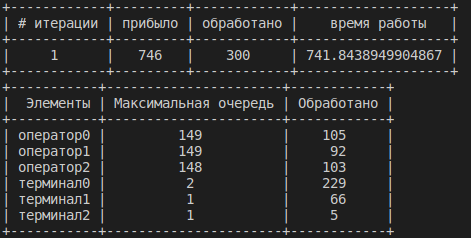
\includegraphics[scale=1.0]{imgs/res1.png}
	\end{center}
	\caption{Работа программы с тремя операторами и тремя терминалами.}
	\label{img:res1}
\end{figure}

Как видно из результатов, операторы не успеваю обработать всех прибывших клиентов, поэтом образуются длинные очереди. 

Добавим еще одного оператора и запустим с теми же параметрами. Результаты работы программы представлены на рисунке \ref{img:res2}

\begin{figure}[H]
	\begin{center}
		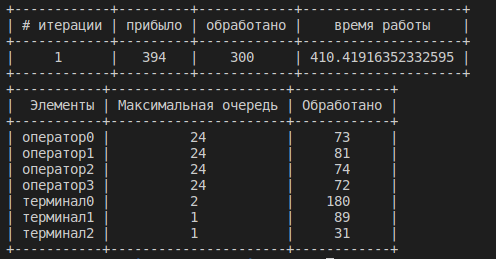
\includegraphics[scale=1.0]{imgs/res2.png}
	\end{center}
	\caption{Работа программы с четыремя операторами и тремя терминалами.}
	\label{img:res2}
\end{figure}

Ситуация становится лучше, но очереди все еще довольно большие. 

Добавим еще двух операторов. Результаты работы программы представлена на рисунке \ref{img:res3}

\begin{figure}[H]
	\begin{center}
		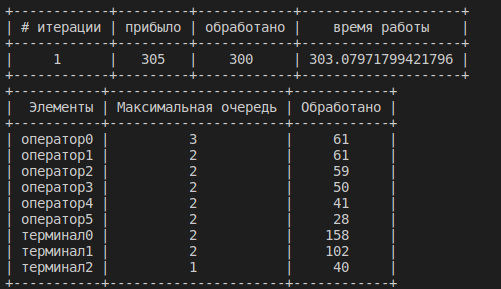
\includegraphics[scale=1.0]{imgs/res3.png}
	\end{center}
	\caption{Результаты работы для 6ти операторов и 3х терминалов.}
	\label{img:res3}
\end{figure}

Как видно из рисунка 4 теперь очереди составляют не больше 3х человек, что приемлимо. 300 человек обслуживаются за 5 часов. 

Также для уменьшения очередей можно улучшить производительность работы операторов. Путь оператор тратит на обслуживание клиента 1-5 минут. А всего операторов 4. Результат работы программы преставлен на рисунке \ref{img:res4}

\begin{figure}[H]
	\begin{center}
		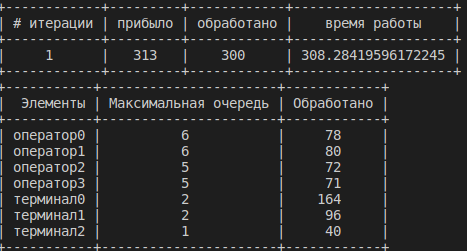
\includegraphics[scale=1.0]{imgs/res4.png}
	\end{center}
	\caption{Работа программы при 4х операторах и трех терминалах с улучшенной эффективностью операторов.}
	\label{img:res4}
\end{figure}

\end{document}